\documentclass{article}
\usepackage{ctex}
\usepackage{graphicx}
\usepackage{amsmath}
\usepackage{geometry}
\usepackage{float}
\geometry{a4paper, margin=1in}

\title{\textbf{系统开发工具基础\_实验报告（第2周）}}
\author{李雨潼 \\ 25020007069}
\date{}

\begin{document}

\maketitle

\section*{一、课上实验题}

\subsection*{第5题：控制一个可清理的后台任务}
\textbf{题目要求：} 将给定的 worker.sh 脚本赋予执行权限，在前台启动，并把 stdout、stderr 分别写入 stdout.log、stderr.log。使用 Ctrl-Z 挂起任务，再用 bg 让它在后台继续；使用 jobs 确认状态。使用 jobs -p 取得 PID，发送 SIGTERM 并等待任务结束。确认 cleanup.log 中出现 CLEAN_EXIT，且任务已经退出。

\textbf{解题过程：} 给脚本添加执行权限并前台运行，按 Ctrl+Z 挂起后用 bg 放入后台，用 jobs 确认状态。通过 jobs -p 获取 PID 后 kill 掉，查看 cleanup.log 确认 CLEAN_EXIT 已写入。

\textbf{执行结果：}
\begin{figure}[H]
    \centering
    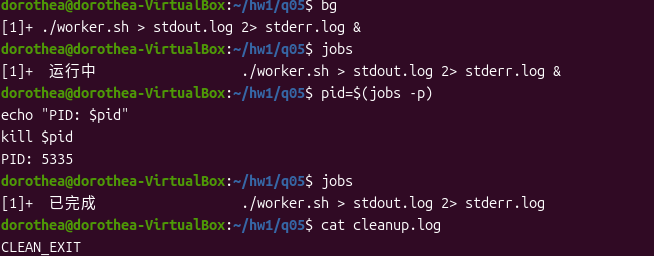
\includegraphics[width=0.9\textwidth]{q5.png}
    \caption{第5题执行结果}
    \label{fig:q5}
\end{figure}

\newpage

\subsection*{第6题：语义重构与本地开发反馈}
\textbf{题目要求：} 在 q06 中按照给定代码创建三个 Python 文件，并使用编辑器语言服务器完成语义重构。分别演示跳转到定义和查找引用。使用"重命名符号"把 total\_price 改为 calculate\_total，保证定义和所有代码引用同步改变。临时加入未使用的 import os，用 ruff 发现并删除；最后运行 ruff 和 pytest 并保证通过。

\textbf{解题过程：} 创建三个 Python 文件，在 VS Code 中演示跳转到定义和查找引用。用重命名符号将 total\_price 改为 calculate\_total，验证三个文件同步更新。临时加入未使用的 import os，用 ruff 发现并自动删除。最后运行 pytest 测试通过。

\textbf{执行结果：}

跳转到定义：
\begin{figure}[H]
    \centering
    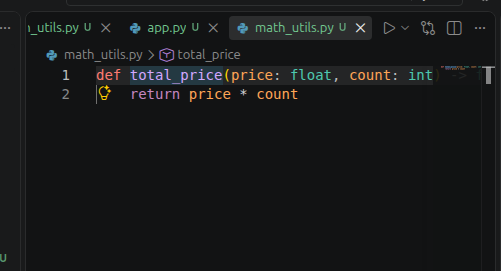
\includegraphics[width=0.9\textwidth]{q6_1.png}
    \caption{跳转到定义}
    \label{fig:q6_1}
\end{figure}

查找引用：
\begin{figure}[H]
    \centering
    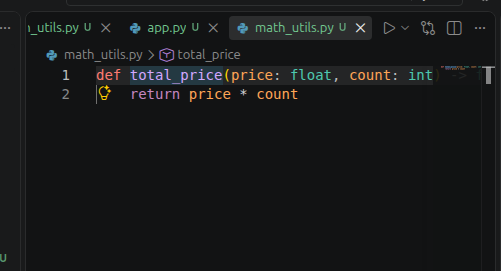
\includegraphics[width=0.9\textwidth]{q6_2.png}
    \caption{查找引用}
    \label{fig:q6_2}
\end{figure}

重命名后三处同步更新：
\begin{figure}[H]
    \centering
    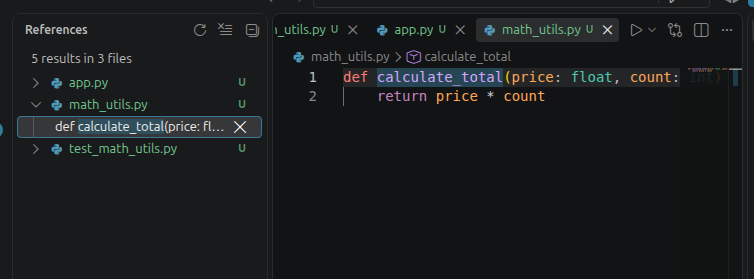
\includegraphics[width=0.9\textwidth]{q6_3.png}
    \caption{math\_utils.py}
    \label{fig:q6_3}
\end{figure}

\begin{figure}[H]
    \centering
    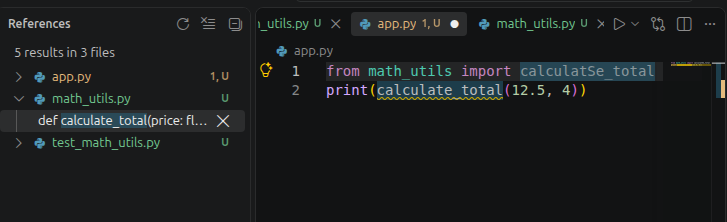
\includegraphics[width=0.9\textwidth]{q6_4.png}
    \caption{app.py}
    \label{fig:q6_4}
\end{figure}

\begin{figure}[H]
    \centering
    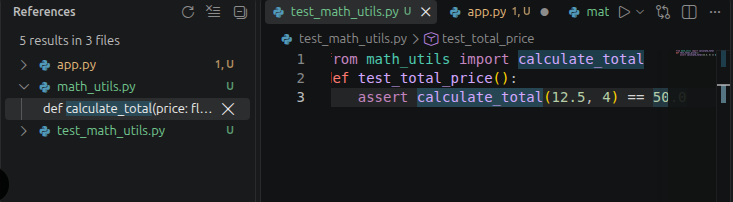
\includegraphics[width=0.9\textwidth]{q6_5.png}
    \caption{test\_math\_utils.py}
    \label{fig:q6_5}
\end{figure}

ruff 检查并修复：
\begin{figure}[H]
    \centering
    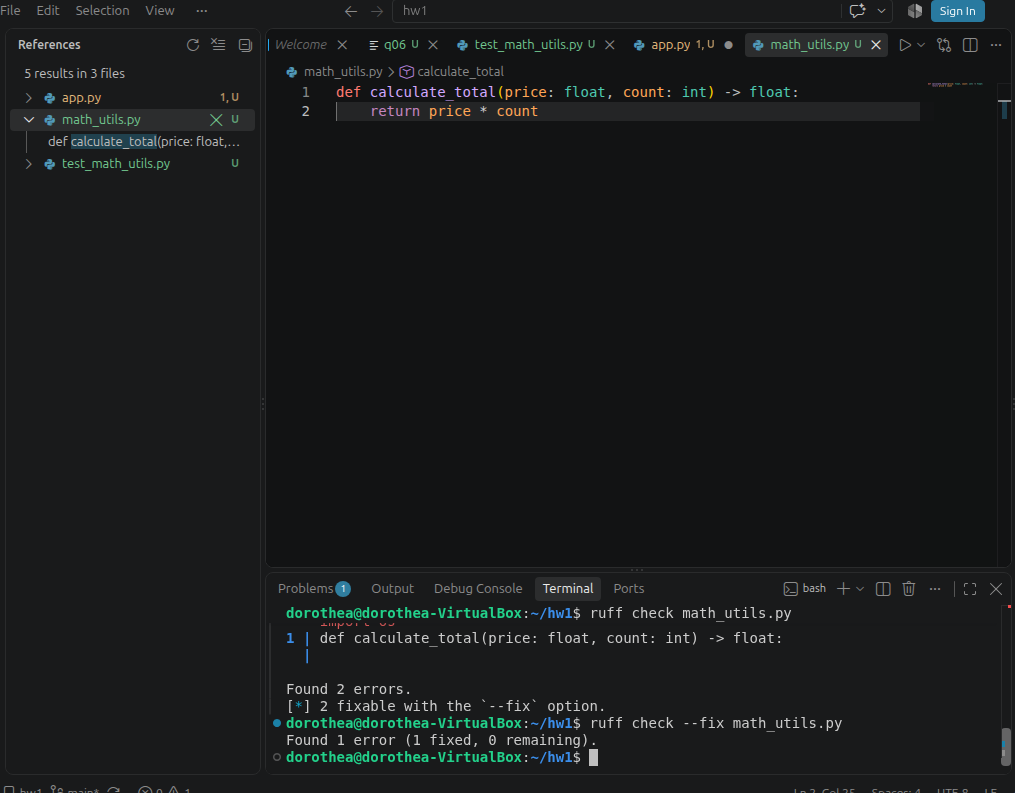
\includegraphics[width=0.9\textwidth]{q6_6.png}
    \caption{ruff 检查结果}
    \label{fig:q6_6}
\end{figure}

pytest 测试通过：
\begin{figure}[H]
    \centering
    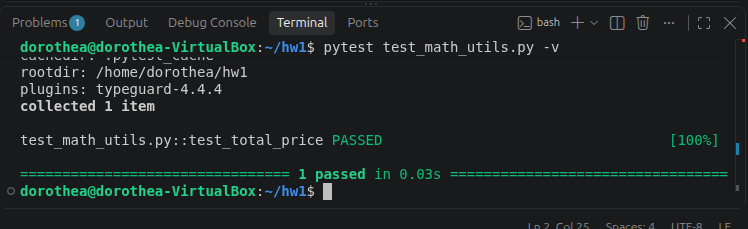
\includegraphics[width=0.9\textwidth]{q6_7.png}
    \caption{pytest 测试通过}
    \label{fig:q6_7}
\end{figure}

\newpage

\subsection*{第7题：用调试器定位并修复排序缺陷}
\textbf{题目要求：} 将给定代码保存为 merge\_sort.py，先运行确认结果错误。使用 pdb 在 merge 中设置断点并观察变量。完成最小修复（不得用 sorted），使用 pytest 增加两个测试并保证通过。

\textbf{解题过程：} 运行发现递归深度超限，将终止条件从 len(a) < 1 改为 <= 1。再运行发现排序结果仍不对，将 merge 函数中的 right[i] 改为 right[j]。修复后用 pdb 设置断点观察变量确认无误。最后写两个 pytest 测试用例全部通过。

\textbf{执行结果：}
\begin{figure}[H]
    \centering
    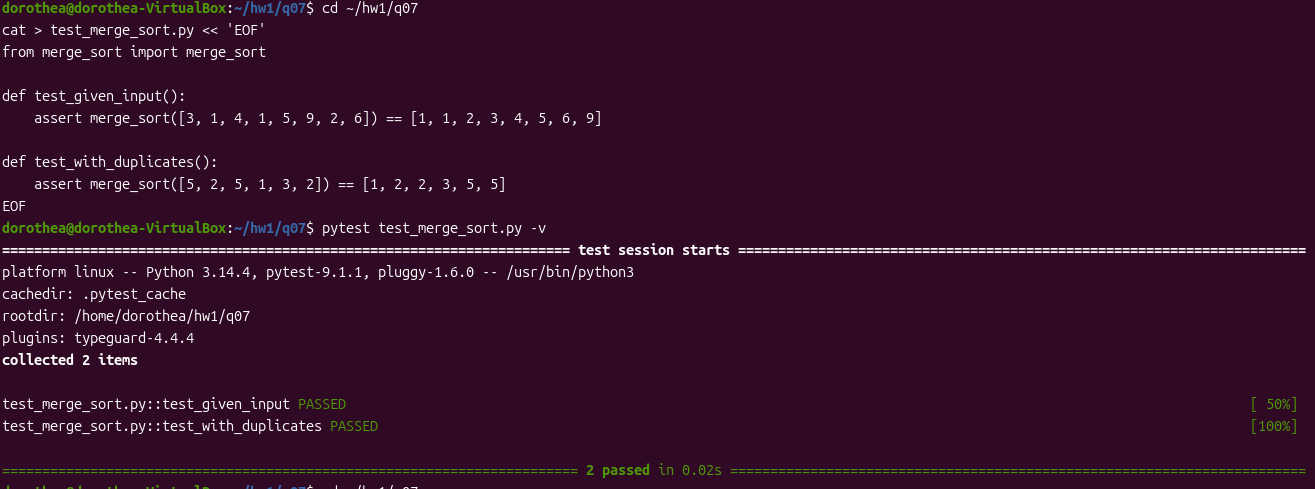
\includegraphics[width=0.9\textwidth]{q7_1.png}
    \caption{正确排序结果及 pytest 测试}
    \label{fig:q7_1}
\end{figure}

\begin{figure}[H]
    \centering
    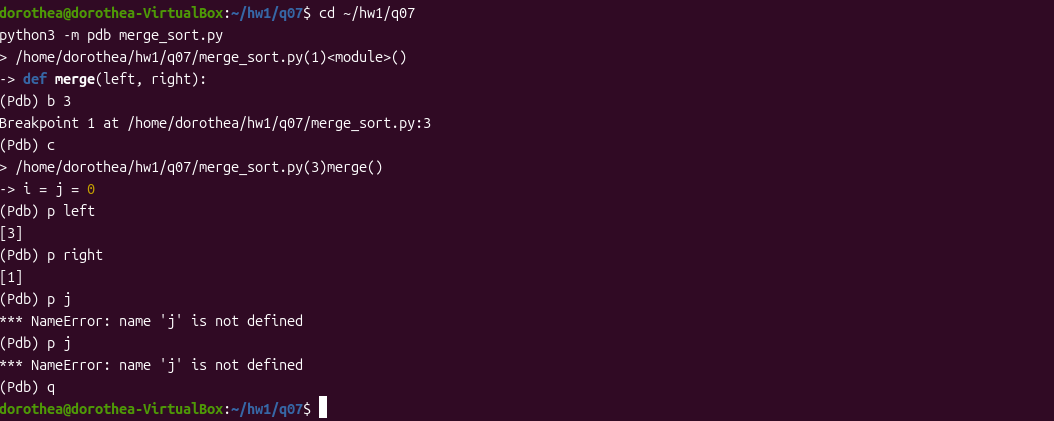
\includegraphics[width=0.9\textwidth]{q7_2.png}
    \caption{pdb 调试过程}
    \label{fig:q7_2}
\end{figure}

\newpage

\subsection*{第8题：先测量再优化慢速词频程序}
\textbf{题目要求：} 生成 words.txt，使用 time 运行原程序 2 次并记录耗时。使用 cProfile 找出性能瓶颈。在不改变最终 count 的前提下优化程序（不得写死 1000），再运行 2 次，计算加速比。

\textbf{解题过程：} 生成 words.txt 后运行原程序，time 测得耗时约 0.119s 和 0.142s。cProfile 分析显示 list 去重是瓶颈，改为 set 去重后耗时降到 0.024s 和 0.032s，加速比约 4.6 倍，count 保持 1000 不变。

\textbf{执行结果：}
\begin{figure}[H]
    \centering
    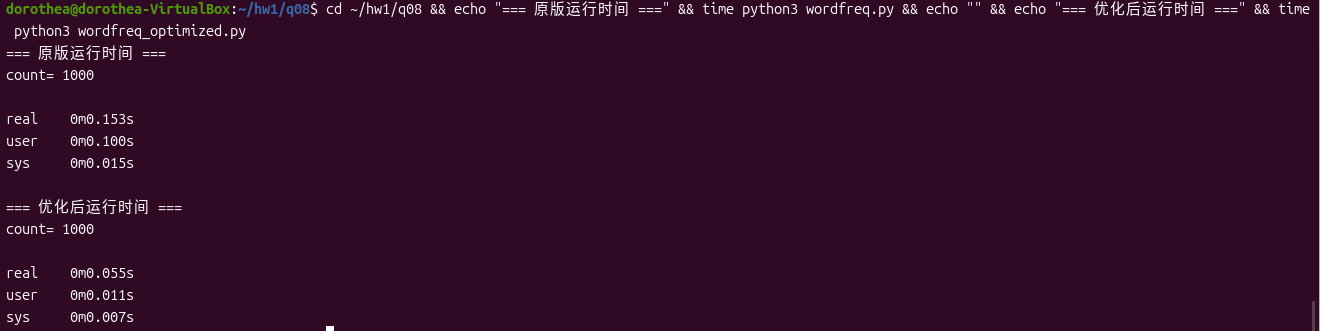
\includegraphics[width=0.9\textwidth]{q8.png}
    \caption{原版与优化版运行时间对比}
    \label{fig:q8}
\end{figure}

\newpage

\section*{二、课后练习（10个实例）}

\subsection*{实例1：特殊参数 -- 的作用}
创建和删除以 -- 开头的文件，验证 -- 可以避免参数被误解析为选项。
\begin{figure}[H]
    \centering
    
\includegraphics[width=0.9\textwidth]{ex1.png}
    \caption{实例1执行结果}
    \label{fig:ex1}
\end{figure}

\subsection*{实例2：自定义 ls 命令}
使用 -lath --color 参数列出文件，显示隐藏文件、易读大小、按时间排序、彩色输出。
\begin{figure}[H]
    \centering
    
\includegraphics[width=0.9\textwidth]{ex2.png}
    \caption{实例2执行结果}
    \label{fig:ex2}
\end{figure}

\subsection*{实例3：进程替换 + diff}
用 diff 比较 printenv 与 export 的输出，观察两者的格式差异。
\begin{figure}[H]
    \centering
    
\includegraphics[width=0.9\textwidth]{ex3.png}
    \caption{实例3执行结果}
    \label{fig:ex3}
\end{figure}

\subsection*{实例4：启用 Vim 模式}
在 Shell 中执行 set -o vi，启用 Vim 风格的命令行编辑模式。
\begin{figure}[H]
    \centering
    
\includegraphics[width=0.9\textwidth]{ex4.png}
    \caption{实例4执行结果}
    \label{fig:ex4}
\end{figure}

\subsection*{实例5：安装 VS Code 扩展}
在 VS Code 中搜索并安装 GitLens 扩展，增强代码浏览体验。
\begin{figure}[H]
    \centering
    
\includegraphics[width=0.9\textwidth]{ex5.png}
    \caption{实例5执行结果}
    \label{fig:ex5}
\end{figure}

\subsection*{实例6：调试归并排序 bug}
修复 merge\_sort 中 right[i] 应为 right[j] 的索引错误。
\begin{figure}[H]
    \centering
    
\includegraphics[width=0.9\textwidth]{ex6.png}
    \caption{实例6执行结果}
    \label{fig:ex6}
\end{figure}

\subsection*{实例7：AddressSanitizer 检测内存错误}
编译时开启 AddressSanitizer，检测到 heap-use-after-free 错误。
\begin{figure}[H]
    \centering
    
\includegraphics[width=0.9\textwidth]{ex7.png}
    \caption{实例7执行结果}
    \label{fig:ex7}
\end{figure}

\subsection*{实例8：strace 追踪系统调用}
用 strace -c ls -l 统计 ls 命令调用的系统调用次数和耗时。
\begin{figure}[H]
    \centering
    
\includegraphics[width=0.9\textwidth]{ex8.png}
    \caption{实例8执行结果}
    \label{fig:ex8}
\end{figure}

\subsection*{实例9：perf 性能分析}
用 perf record 采集 slow.c 的运行数据，再用 perf report 查看热点函数。
\begin{figure}[H]
    \centering
    
\includegraphics[width=0.9\textwidth]{ex9.png}
    \caption{实例9执行结果}
    \label{fig:ex9}
\end{figure}

\subsection*{实例10：查找并终止占用端口的进程}
启动 http.server 占用 4444 端口，用 ss 查找并 kill 终止。
\begin{figure}[H]
    \centering
    
\includegraphics[width=0.9\textwidth]{ex10.png}
    \caption{实例10执行结果}
    \label{fig:ex10}
\end{figure}

\newpage

\section*{三、解题感悟}

本次实验涵盖了命令行环境、开发工具、调试和性能分析四个主题。

第5题让我熟悉了 Shell 的任务控制和信号处理，通过 bg、jobs、kill 等命令管理后台进程。第6题展示了编辑器语言服务器的功能，跳转定义、查找引用和重命名符号提高了代码维护效率。第7题的调试练习让我学会了用 pdb 逐步跟踪变量状态。第8题通过 cProfile 和 time 直观看到了 set 去重相比 list 去重的性能提升。

课后10个实例补充了 strace、perf、AddressSanitizer 等工具的使用，这些在日常开发和调试中都很实用。整体来说，这周实验让我对各种开发工具有了更具体的认识。

\end{document}